% Chapter Template

\chapter{Introducción} % Main chapter title

\label{Chapter1} % Change X to a consecutive number; for referencing this chapter elsewhere, use \ref{ChapterX}

\lhead{Capítulo 1. \emph{Introducción}} % Change X to a consecutive number; this is for the header on each page - perhaps a shortened title


\section{Introducción}

Lorem ipsum dolor sit amet, consectetur adipiscing elit. Integer congue magna eu tortor hendrerit commodo. Integer consectetur, ante ut venenatis volutpat, turpis diam venenatis massa, id tincidunt ligula velit porta quam. Mauris vel auctor lorem. Vestibulum nisl lorem, ultricies a commodo at, semper quis erat. Aenean pharetra felis lectus, id blandit mauris congue non. Vestibulum efficitur sagittis dui, ut feugiat elit pretium sed. Donec viverra, lacus sed dictum pellentesque, lectus mauris ultricies arcu, vel vestibulum velit erat vitae elit. Phasellus quis aliquam neque. Nunc placerat molestie dui id sollicitudin. Duis odio mi, rhoncus eget lobortis nec, ornare at leo.



%----------------------------------------------------------------------------------------
%	SECTION 1
%----------------------------------------------------------------------------------------

\section{Lorem Ipsum}

Integer faucibus malesuada luctus. Vestibulum pellentesque imperdiet luctus. Fusce urna leo, faucibus vitae condimentum ut, rutrum rhoncus neque. Maecenas dignissim nisl id ultrices tincidunt. Donec consectetur in est at auctor. Ut luctus finibus lacus, sit amet consectetur purus euismod eget. Sed lacinia consequat placerat. Donec pretium orci non justo consequat dignissim.\\

\begin{figure}[htbp]
	\centering
		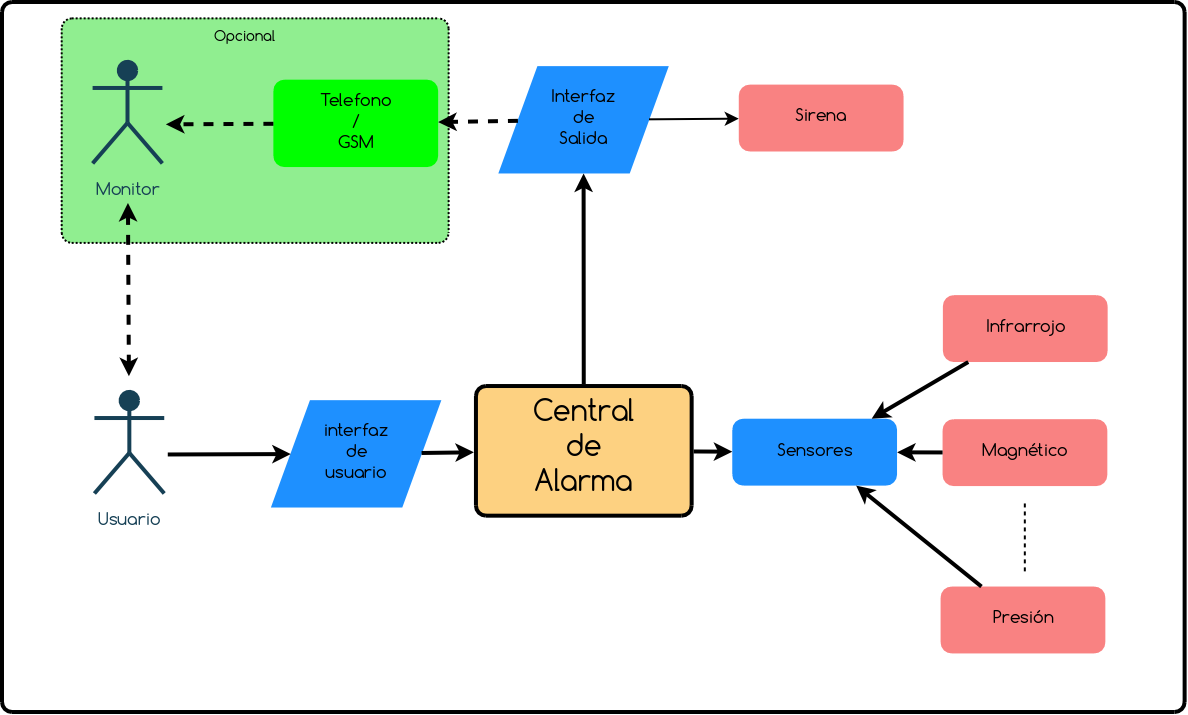
\includegraphics[width=1\textwidth]{Figures/Diagrama_clasico.png}
		\rule{35em}{1pt}
	\caption[Esquema clásico de Seguridad]{Esquema clásico de Seguridad}
	\label{fig:Diagrama_clasico}
\end{figure}

\newpage
%-----------------------------------
%	SUBSECTION 1.1
%-----------------------------------
\subsection{Neque porro quisquam}
Vestibulum id lacus viverra, placerat sem vitae, porta lacus. Proin semper, purus et faucibus feugiat, massa tortor lacinia ex, non dapibus enim turpis eget tortor. Duis vel purus viverra, aliquam sem consequat, efficitur nisl. Quisque elementum at nulla vitae tincidunt. Maecenas sagittis lacinia mi, quis mollis ante pulvinar eu. Mauris ut pellentesque augue. Donec non libero blandit, venenatis sem scelerisque, faucibus mi.

\begin{itemize}
\item Nullam consectetur.
\item libero at facilisis dapibus.
\end{itemize}

\subsubsection{Consectetur, adipisci}
Nullam consectetur, libero at facilisis dapibus, libero justo semper nulla, ut mattis arcu ante non justo. Aenean ultrices convallis erat in mollis. Pellentesque eu consectetur enim. Maecenas at congue quam. Lorem ipsum dolor sit amet, consectetur adipiscing elit. Fusce egestas orci orci, non sodales nunc malesuada sed. Donec vel quam id lacus dictum ultrices. Nullam dignissim nunc vitae iaculis sodales. Etiam sed velit non dui viverra feugiat.